% Chapter 2

\chapter{Analysis Strategy} \label{Chapter2}

The purpose of this analysis is to search for a heavy resonance decaying into a $Z$ boson and a Higgs boson. The $Z$ boson is reconstructed from the dielectron or dimuon final state. The $Z\rightarrow l^+l^-$ channel is chosen mainly because it has low QCD and $t\bar{t}$ backgrounds. The Higgs boson is reconstructed via the $b\bar{b}$ channel because the branching ratio of \Hbb is the largest at $m_H$ = 125 GeV. Note that the $b$ quarks are reconstructed as a single jet with large radius in the CMS detector due to the high transverse momentum of Higgs.

In this chapter, the data sets and Monte Carlo (MC) samples used are presented, and the selection criteria of physics objects are introduced. The final selection efficiency is also discussed and reported. The data and MC comparisons of various kinematic variables are presented to show the agreement between them.

\section{Data Sets and Monte Carlo Samples} 

\subsection{Data Sets}

In this analysis, the data collected with CMS during 2015 RunD, with integrated luminosity of 2.51 $fb^{-1}$ are used. The muon and electron data sets are collected with a single-muon or a single-electron trigger, which will be explained in detail in latter section. All data sets used are listed in Table~\ref{tab:dataSample}. Moreover, a list of filters~\cite{filters} are applied on data in order to remove problematic or noise-dominated events, are reported in Table~\ref{tab:filter}.

\begin{table}[t]
  \caption{Data sets Run2015D used in this analysis.}
  \label{tab:dataSample}
  \centering
  \begin{tabular}{c c}
    \toprule
    \tabhead{Samples} & \tabhead{Luminosity $L$ [$fb^{-1}$]} \\
    \midrule
    SingleElectron-Run2015D-05Oct2015-v1  & 0.877 \\
    SingleElectron-Run2015D-PromptReco-v4 & 1.635 \\
    \midrule
    SingleMuon-Run2015D-05Oct2015-v1      & 0.877  \\
    SingleMuon-Run2015D-PromptReco-v4     & 1.635  \\
    \bottomrule                                    \\
  \end{tabular}
\end{table}

\begin{table}[t]
  \caption{Filters used in this analysis.}
  \label{tab:filter}
  \centering
  \begin{tabular}{c}
    \toprule
    Filters            \\
    \midrule
    CSCTightHaloFilter \\
    eeBadScFilter      \\
    HBHENoiseFilter    \\
    HBHENoiseIsoFilter \\
    \bottomrule        \\
  \end{tabular}
\end{table}

\subsection{Monte Carlo Samples}

\subsubsection*{Signal samples}

The signal samples are generated with the \texttt{MadGraph5}~\cite{Alwall:2011uj} LO generator. The showering and hadronization have been performed with \texttt{PYTHIA8}~\cite{Sjostrand:2007gs}. A full detector simulation and event reconstruction has been performed with \texttt{GEANT4}~\cite{Agostinelli:2002hh} and \texttt{CMSSW}. The simulated signal MC samples are listed in Table~\ref{tab:signalSample}. All signal samples belong to the \texttt{RunIISpring15MiniAODv2-74X\_mcRun2} campaign with the 25 ns asymptotic conditions. Moreover, the samples are produced assuming the narrow-width approximation, with the resonance width set to 1 MeV.

\subsubsection*{Background samples}

All physics processes yielding final states with one or two leptons in association with one or two $b$ quarks are considered as possible sources of background for the analysis. The list of background samples used is reported in Table~\ref{tab:bkgSample}.

The \Zjets background is produced in several samples binned in $H_T$ (the scalar sum of the $p_T$ of the outgoing partons) starting from 100 GeV with the \texttt{MadGraph5} LO generator. The contribution of events with $H_T$ less than 100 GeV is found to be negligible after requiring the $Z$ $p_T$ to be greater than 200 GeV. The inclusive $t\bar{t}$ sample has been produced with \texttt{POWHEG}~\cite{Oleari:2010nx} interfaced with \texttt{PYTHIA8}, including all the possible decays of the W bosons. For the diboson production processes, the $WW$, $WZ$, and $ZZ$ are inclusive processes generated with \texttt{PYTHIA8}, while the $ZH$ has decay mode same as the decay mode of signal and is generated with \texttt{POWHEG}.

The cross sections listed in the table are used to normalize SM backgrounds. The cross sections of \Zjets samples are computed by \texttt{MadGraph5} with an NLO/LO electroweak correction~\cite{Kallweit:2015dum} (k-factor) derived from the inclusive $Z$ cross section computed by \texttt{FEWZ}~\cite{Gavin:2010az}. The amount of k-factor as a function of the $Z$ $p_T$ is presented in Figure~\ref{fig:EWfactor}. The cross section of $t\bar{t}$ samples are obtained from TTbarNNLO group~\cite{Khachatryan:2015oqa}, while the $VV$ samples are computed from \texttt{MCFM}~\cite{Campbell:2010ff} calculator.

\begin{figure}[t]
  \centering
  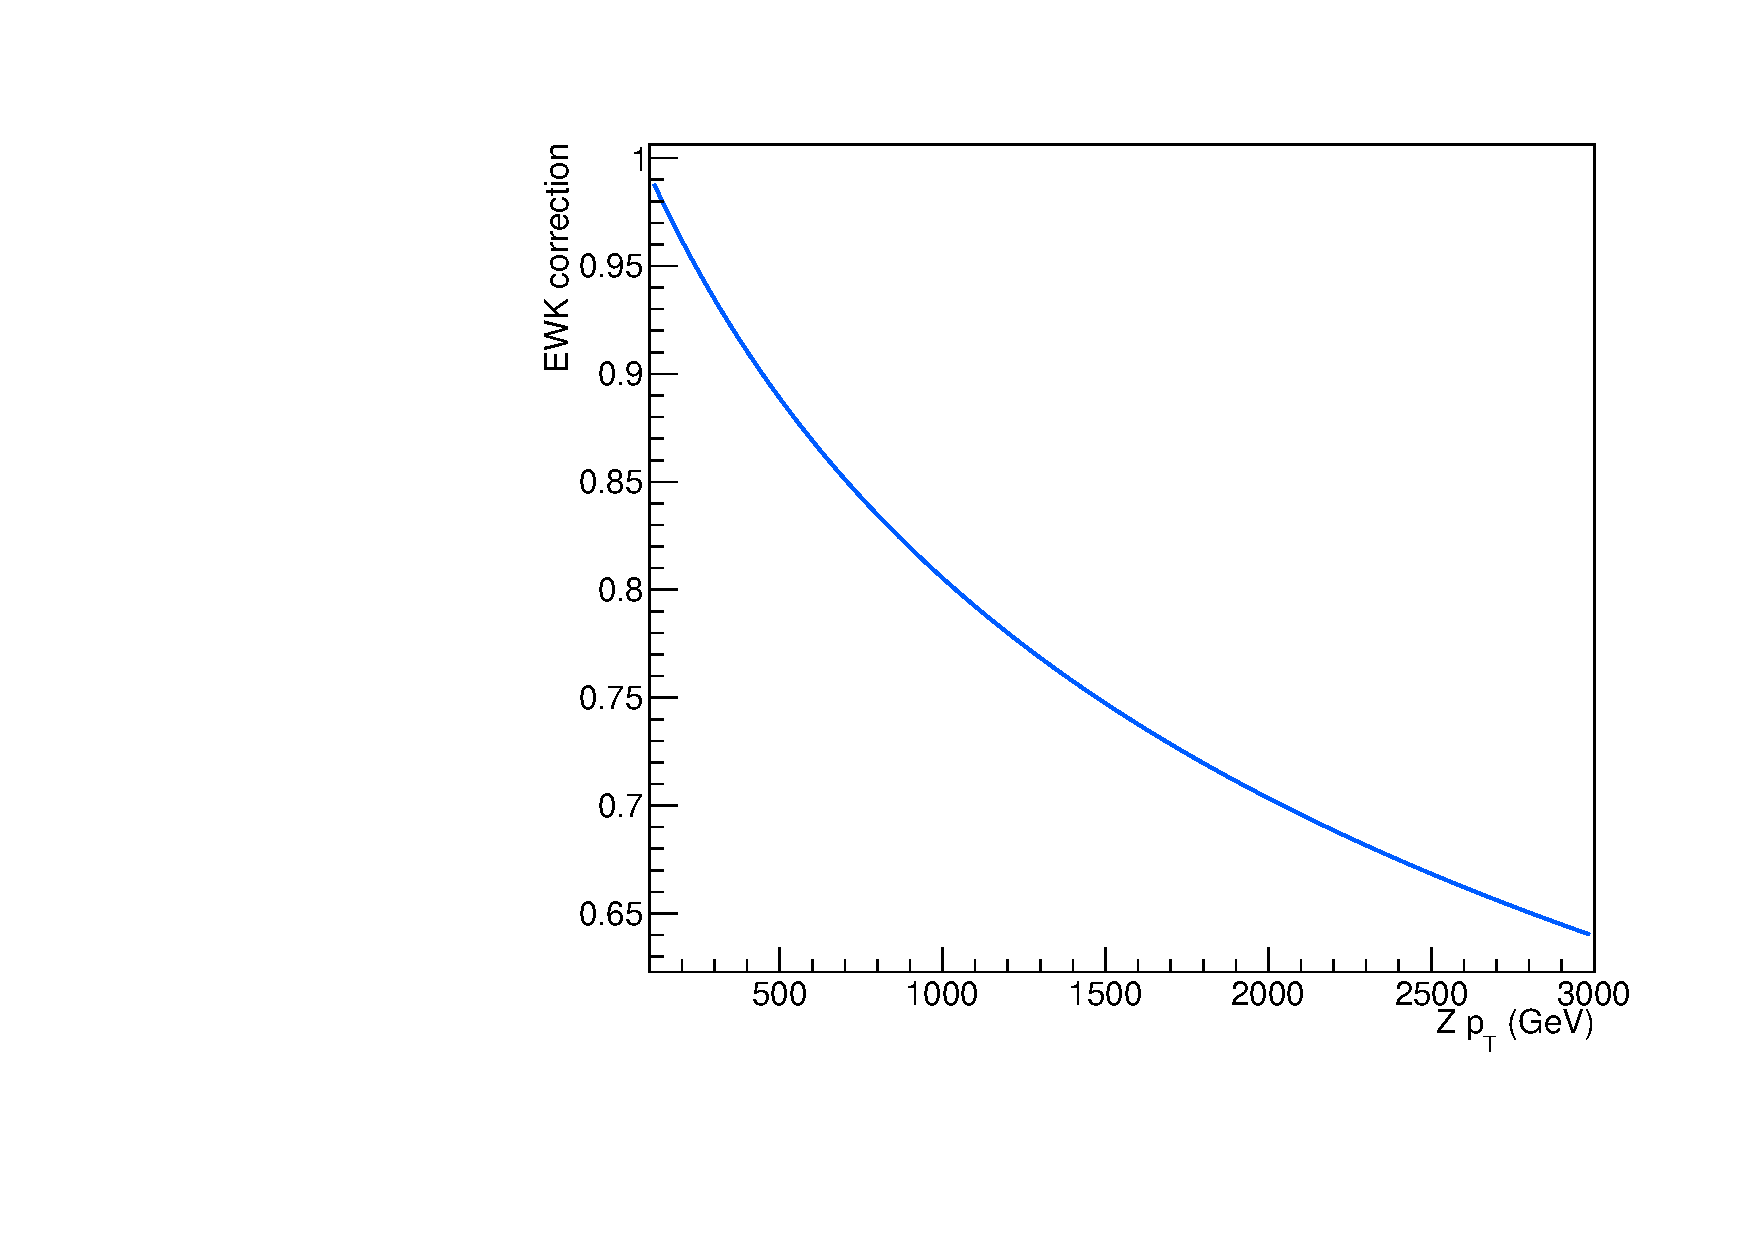
\includegraphics[width=0.75\textwidth]{Figures/EWfactor.pdf}
  \caption{Electroweak correction for the $Z$ as a function of the transverse momentum.}
  \label{fig:EWfactor}
\end{figure}

\begin{sidewaystable}
  \caption{Signal samples used in this analysis.}
  \label{tab:signalSample}
  \centering
  \begin{tabular}{c c c}
    \toprule
    \tabhead{Samples} & \tabhead{Number of events} & \tabhead{Cross section $\sigma$ [$pb$]} \\
    \midrule
    ZprimeToZhToZlephbb\_narrow\_M-800\_13TeV-madgraph-v1  & 48400 & 0.0282665     \\
    ZprimeToZhToZlephbb\_narrow\_M-1000\_13TeV-madgraph-v1 & 50000 & 0.0153743     \\
    ZprimeToZhToZlephbb\_narrow\_M-1200\_13TeV-madgraph-v1 & 50000 & 0.00790857    \\
    ZprimeToZhToZlephbb\_narrow\_M-1400\_13TeV-madgraph-v1 & 50000 & 0.00421385    \\
    ZprimeToZhToZlephbb\_narrow\_M-1600\_13TeV-madgraph-v1 & 50000 & 0.00233319    \\
    ZprimeToZhToZlephbb\_narrow\_M-1800\_13TeV-madgraph-v1 & 50000 & 0.00133522    \\
    ZprimeToZhToZlephbb\_narrow\_M-2000\_13TeV-madgraph-v1 & 50000 & 0.000785119   \\
    ZprimeToZhToZlephbb\_narrow\_M-2500\_13TeV-madgraph-v1 & 50000 & 0.000227178   \\
    ZprimeToZhToZlephbb\_narrow\_M-3000\_13TeV-madgraph-v1 & 50000 & 0.000071426   \\
    ZprimeToZhToZlephbb\_narrow\_M-3500\_13TeV-madgraph-v1 & 49800 & 0.0000235715  \\
    ZprimeToZhToZlephbb\_narrow\_M-4000\_13TeV-madgraph-v1 & 49800 & 0.00000797489 \\
    \bottomrule \\
  \end{tabular}
\end{sidewaystable}

%%%%%%%%
\begin{figure}[t]
  \centering
  \foreach \n in {5,6}{
    \begin{tabular}{ll}
      \includegraphics[page=\n,width=0.375\textwidth]{Figures/dataMCcompare/eleZjetVariable.pdf} &
      \includegraphics[page=\n,width=0.375\textwidth]{Figures/dataMCcompare/muZjetVariable.pdf} \\
    \end{tabular}
  }
  \caption{Distributions of $p_T$ and $\eta$ variable for the leading leptons of $Z$ candidate in electron channel (left) and in muon channel (right).}
  \label{fig:dataMC_Zlead}
\end{figure}
